% -*- mode: fundamental -*-

% ****************************************************************

\chapter{BSV Finite State Machines for the RISC-V Fetch step}

\markboth{Ch \arabic{chapter}: FSM Fetch (DRAFT)}{\copyrightnotice}

\setcounter{page}{1}
% \renewcommand{\thepage}{\arabic{page}}
\renewcommand{\thepage}{\arabic{chapter}-\arabic{page}}

\label{ch_FSM_Fetch}

% ****************************************************************

\section{Introduction}

In this chapter we focus on learning enough BSV to code the front part
of the algorithm shown in Figure~\ref{Fig_Simple_Instr_Exec}, which we
repeat here for convenience.
\begin{figure}[htbp]
  \centerline{\includegraphics[width=6in,angle=0]{ch030_RISCV_Design_Space/Figures/Fig_Simple_Instr_Exec}}
  \caption{\label{Fig_FSM_Fetch_Simple_Instr_Exec}Simple interpretation of RISC-V instructions (same as Fig.~\ref{Fig_Simple_Instr_Exec})}
\end{figure}
We have
already seen the Decode function in the previous chapter.  Now we will
add the Read-PC-and-Fetch functionality, and then place this, along
with the Decode function, into a Finite State Machine that will
continually fetch and decode instructions.

The outputs of Read-PC-and-Fetch step are:
\begin{tightlist}

 \item A \emph{memory request} to memory, to read an instruction.

 \item Some additional information passed on to the Decode step for subsequent use.

\end{tightlist}

% ****************************************************************

\section{RISC-V: Memory Requests}

\index{Memory!Request}

A memory-request is either for reading data (``load'') or for writing
data (``store'').  We express these request-types using an enum type:

\begin{Verbatim}[frame=single, numbers=left]
typedef enum {MEM_LOAD,
	      MEM_STORE} Mem_Req_Type
deriving (Eq, FShow, Bits);
\end{Verbatim}

A memory-request in RISC-V RV32I may be for one, two or four bytes.
We express these request-size options using an enum type:

\begin{Verbatim}[frame=single, numbers=left]
typedef enum {MEM_1B, MEM_2B, MEM_4B} Mem_Req_Size
deriving (Eq, FShow, Bits);
\end{Verbatim}

Finally, a memory request bundles a request type, a size, and an
address.  For memory-writes, we also bundle the data to be stored.  We
express this bundle using a struct:

\begin{Verbatim}[frame=single, numbers=left]
typedef struct {Mem_Req_Type  req_type;
		Mem_Req_Size  size;
		Bit #(XLEN)   addr;
		Bit #(XLEN)   data;    // Only for STORE
} Mem_Req
deriving (Eq, FShow, Bits);
\end{Verbatim}

For STORE requests of 1 and 2 bytes, we assume the data is passed in
the least-significant bytes of the data field.

This is the information sent to Memory from the Read-PC-and-Fetch step
and also from the Execute-Memory-Ops step in
Figure~\ref{Fig_FSM_Fetch_Simple_Instr_Exec}.

% ****************************************************************

\section{RISC-V: Address Alignment}

\index{Address alignment}
\index{Memory!Address alignment}

Although nowadays we think of all computer memories in units of bytes,
and being byte-addressed, in practice in hardware, it is usually
simpler if memory-requests are \emph{aligned} to an address according
to the request-size.  Specifically, the address for a 2-byte request
should be even, {\ie} the least significant bit of the address,
\verb|addr[0]|, should be zero.  The address for a 4-byte request
should have zero in the two least significant bits (\verb|addr[1:0]|).

We can see why address-alignment is desirable.  In a memory organized
according to wider words, a misaligned read request may straddle word
boundaries and so may require reading two words.  In a memory system
with caches, a misaligned read request may straddle a cache-line
boundary, and may require two accesses, which may hit or miss
independently.  In a memory system with virtual memory, a misaligned
read request may straddle a page boundary, and may require two
accesses, which may hit or page-fault independently.  In short,
misaligned accesses add complexity to memory-system hardware design.

We can organize our software so that misaligned accesses are
exceedingly rare.  Since most software is produced by compilers, we
can make the compiler ensure that instructions and data are placed in
memory at aligned addresses, possibly by padding gaps between
``adjacent'' small data (such as two byte-sized fields in a struct).

Rather than paying the price of additional complexity to handle
misaligned accesses, to be used only in rare cases when accesses are
actually misaligned, memory-system designers usually choose instead to
return an error on misaligned accesses.  The error will cause the CPU
to ``trap'', and special trap-handling code can then recover by
explicitly performing two, smaller, aligned accesses.

% ****************************************************************

\section{RISC-V: Memory Responses}

\index{Memory!Response}

The response from memory for a any request may be to report success,
an alignment error, or some other error.  Examples of ``other errors''
are:

\begin{tightlist}

\item Absence of memory at the given address ({\eg}, although RV32I
  addresses are 32-bits, which can address 4GiB of memory, we may
  provision our system with something smaller, say 1 GiB);

\item Corruption of data, as detected by parity bits or some other
  error-detection mechanism).

\end{tightlist}

These different memory response-types can be encoded in an enum type:

\begin{Verbatim}[frame=single, numbers=left]
typedef enum {MEM_OK, MEM_MISALIGNED, MEM_ERR} Mem_Rsp_Type
deriving (Eq, FShow, Bits);
\end{Verbatim}

A memory-response contains the response-type and, for LOAD requests
that with OK response-type, the data that was read from memory.  This
can be expressed in a struct:

\begin{Verbatim}[frame=single, numbers=left]
typedef struct {Mem_Rsp_Type  rsp_type;
		Bit #(XLEN)   data;    // Only for LOAD
} Mem_Rsp
deriving (Eq, FShow, Bits);
\end{Verbatim}

For LOAD requests of 1 and 2 bytes, we assume the data is passed in
the least-significant bytes of the data field.

// ****************************************************************

\section{RISC-V: more structs for the Fetch function}

In Figure~\ref{Fig_FSM_Fetch_Simple_Instr_Exec}, the information
passed from the Fetch stage to the Decode stage is just the PC:

\begin{Verbatim}[frame=single, numbers=left]
typedef struct {
   Bit #(XLEN) pc;
} F_to_D
deriving (Bits, FShow);
\end{Verbatim}

\index{BSV!struct!Single-field structs}

It might seem like overkill to define a struct for just one field like
this, but it has the following advantages:

\begin{itemize}

  \item It becomes easy to add more fields later, should we need to do
    so.  In particular for Fife will will need to add some
    branch-prediction information.  We may also wish to add temporary
    fields that aid in debugging.

  \item Stronger type-checking: each new struct type is distinct from
    all other types in a BSV program.  Thus, the type-checker will
    catch any error where we may inadvertantly pass some irrelevant
    32-bit value in place of an \verb|F_to_D| struct.

  \item And \verb|F_to_D| value occupies the same XLEN bits as the
    \verb|pc| field by itself; there is no overhead just because we
    used a struct.

\end{itemize}

\index{BSV!struct!Nested}

Structs can be nested.  The Fetch function's result is a nested struct
containing two structs, one being the memory-request to be sent to
memory, and the other being the information to be passed on to the
Decode step:

\begin{Verbatim}[frame=single, numbers=left]
typedef struct {
   F_to_D   to_D;
   Mem_Req  mem_req;
} Result_F
deriving (Bits, FShow);
\end{Verbatim}

% ****************************************************************

\section{RISC-V: The Fetch Function}

\label{Sec_FSM_Fetch_Fn_F}

Finally, we are ready to write the Fetch function.  Its input is the
current value of the program counter (PC), and it returns a
\verb|Result_F|.  The PC is used as the address from which to read
memory.

\begin{Verbatim}[frame=single, numbers=left]
function Result_F fn_F (Bit #(XLEN)  pc)
    Result_F y = ?;

    // Info to next stage
    y.to_D = F_to_D {pc: pc};

    // Request to IMem
    y.mem_req = Mem_Req {req_type: MEM_LOAD,
                         size:     MEM_4B,
                         addr:     pc,
                         data :    0};
      return y;
endfunction
\end{Verbatim}

% ****************************************************************

\section{BSV: Memory for our RISC-V CPU}

\index{BSV!Memory}

% ****************************************************************

\section{BSV: Finite State Machines (FSMs)}

\index{BSV!FSM}

% ****************************************************************

\section{RISC-V: Partial CPU with Fetch and Decode}

\index{BSV!FSM}

% ****************************************************************

\section{Topics}

\begin{tightlist}

\item CPU state machine

\item Top-level, connecting to memory

\end{tightlist}

% ****************************************************************
